\begin{table}[!ht]
	\centering
	\caption{Results averaged over $n=10$ iterations (mean $\pm$ std. dev.).}
	\label{tab:results}
	\resizebox{\textwidth}{!}{%
		\begin{tabular}{c|ccc|c|cc|ccc}
			Dataset  & $B$ & $D$ & $D'$ & $\bar{S}_e$ & $\bar{\mathcal{L}}_0$ & $\bar{\mathcal{L}}_1$ & $c^*$ & $\bar{\mathcal{L}}_0'$ & $\bar{\mathcal{L}}_1'$  \\ \hline
			Polbooks & 3 & 3 & -- & $2.250 \pm 0.000$ & $0.563 \pm 0.042$ & $0.595 \pm 0.089$ & -- & -- & -- \\
			School & 10 & 13 & 10 & $1.894 \pm 0.004$ & $0.787 \pm 0.127$ & $0.885 \pm 0.129$ & $1.198 \pm 0.249$ & $0.793 \pm 0.132$ & $0.853 \pm 0.132$ \\
			FB egonet & 10  & 480 & 10 & $1.626 \pm 0.003$ & $1.326 \pm 0.043$ & $1.538 \pm 0.069$ & $0.94 \pm 0.019$ & $1.580 \pm 0.150$ & $1.605 \pm 0.106$
		\end{tabular}
	}
\end{table}

\begin{figure}[!ht]
	\centering
	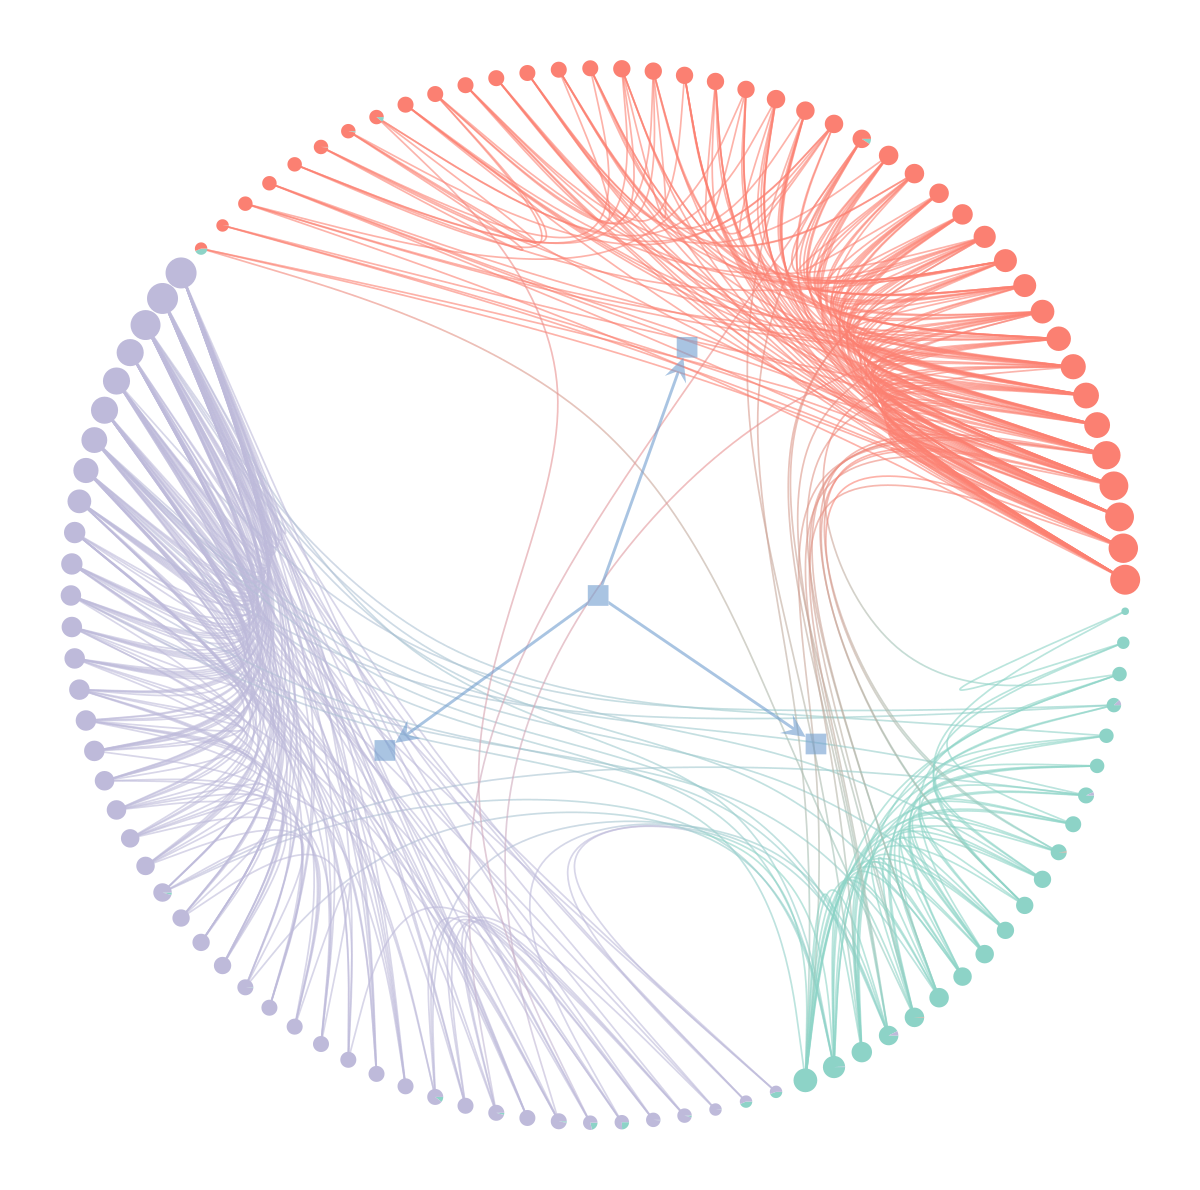
\includegraphics[width=0.28\linewidth]{img/polbooks-graph.png}
	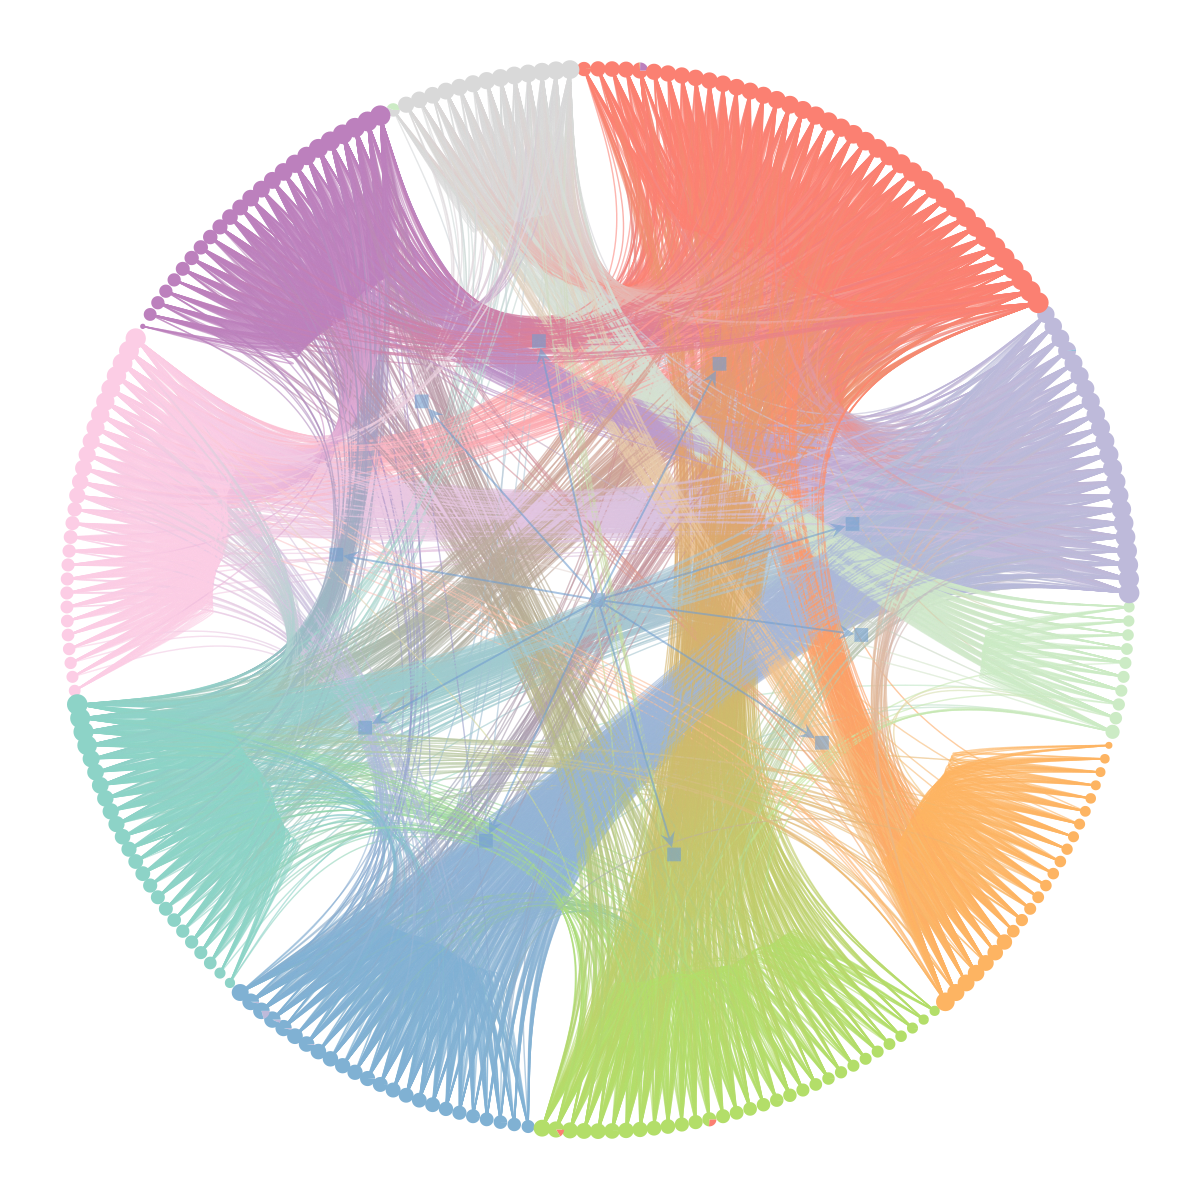
\includegraphics[width=0.28\linewidth]{img/school-graph.png}
	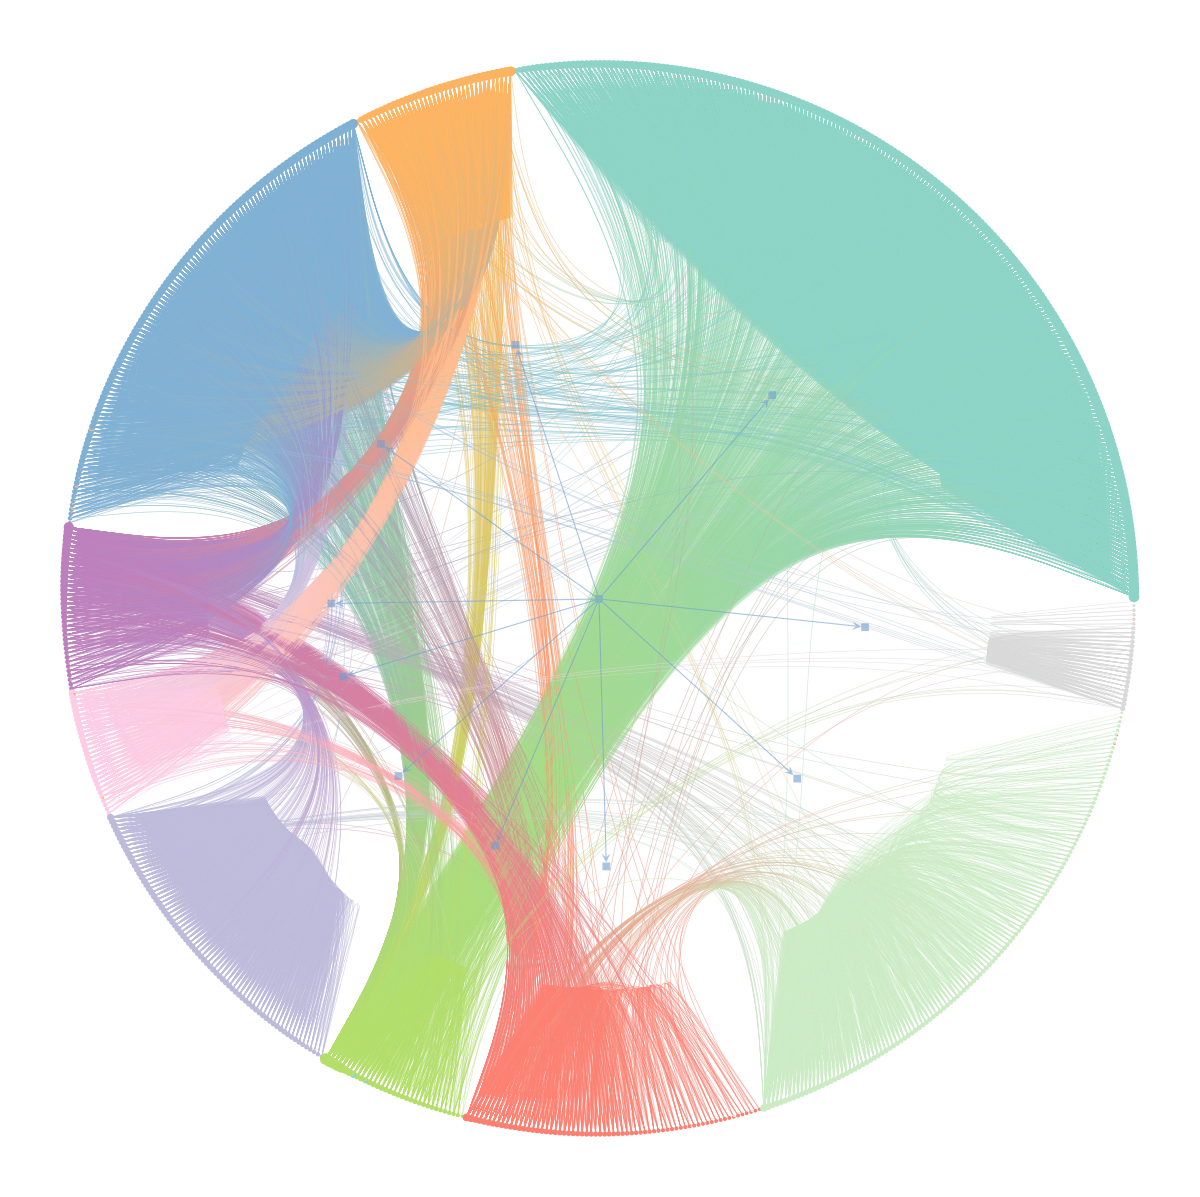
\includegraphics[width=0.28\linewidth]{img/fb-graph.png}
	\caption{Networks laid out and coloured according to inferred block memberships. Left to right: Polbooks, Krebs (2004); Primary School, Stehle et al (2011); Facebook Egonet, Leskovec and Mcauley (2012).}
	\label{fig:graphs-all}
\end{figure}
